\documentclass[a4paper, 12pt, slovene]{article}
\usepackage[slovene]{babel}
\usepackage[utf8]{inputenc}
\usepackage{lmodern}
\usepackage[T1]{fontenc}
\usepackage{graphicx}
\usepackage{caption}
\captionsetup{font=footnotesize}
\usepackage{fullpage}
\usepackage{enumitem}
\usepackage{array}
\usepackage{wrapfig}
\usepackage{multirow}
\usepackage{tabularx}
\usepackage{amsmath}
\usepackage{amssymb}
\usepackage{subcaption}
\newcommand*\diff{\mathop{}\!\mathrm{d}}
\newcommand*\Diff[1]{\mathop{}\!\mathrm{d^#1}}
\newcommand*\difft{\mathop{}\!\ddot{ }}
\usepackage{float}
\usepackage{mathrsfs}
\usepackage{fancyvrb}
\usepackage{hyperref}
\usepackage{xurl}
\usepackage{breqn}

\numberwithin{equation}{section}
\newcommand{\Ai}{\mathrm{Ai}}
\newcommand{\Bi}{\mathrm{Bi}}

\renewcommand{\Re}{\mathop{\rm Re}\nolimits}
\renewcommand{\Im}{\mathop{\rm Im}\nolimits}
\newcommand{\Tr}{\mathop{\rm Tr}\nolimits}
\newcommand{\diag}{\mathop{\rm diag}\nolimits}
\newcommand{\dd}{\,\mathrm{d}}
\newcommand{\ddd}{\mathrm{d}}
\newcommand{\ii}{\mathrm{i}}
\newcommand{\lag}{\mathcal{L}\!}
\newcommand{\ham}{\mathcal{H}\!}
\newcommand{\four}[1]{\mathcal{F}\!\left(#1\right)}
\newcommand{\bigO}[1]{\mathcal{O}\!\left(#1\right)}
\newcommand{\sh}{\mathop{\rm sinh}\nolimits}
\newcommand{\ch}{\mathop{\rm cosh}\nolimits}
\renewcommand{\th}{\mathop{\rm tanh}\nolimits}
\newcommand{\erf}{\mathop{\rm erf}\nolimits}
\newcommand{\erfc}{\mathop{\rm erfc}\nolimits}
\newcommand{\sinc}{\mathop{\rm sinc}\nolimits}
\newcommand{\rect}{\mathop{\rm rect}\nolimits}
\newcommand{\ee}[1]{\cdot 10^{#1}}
\newcommand{\inv}[1]{\left(#1\right)^{-1}}
\newcommand{\invf}[1]{\frac{1}{#1}}
\newcommand{\sqr}[1]{\left(#1\right)^2}
\newcommand{\half}{\frac{1}{2}}
\newcommand{\thalf}{\tfrac{1}{2}}
\newcommand{\pd}{\partial}
\newcommand{\Dd}[3][{}]{\frac{\ddd^{#1} #2}{\ddd #3^{#1}}}
\newcommand{\Pd}[3][{}]{\frac{\pd^{#1} #2}{\pd #3^{#1}}}
\newcommand{\avg}[1]{\left\langle#1\right\rangle}
\newcommand{\norm}[1]{\left\Vert #1 \right\Vert}
\newcommand{\braket}[2]{\left\langle #1 \vert#2 \right\rangle}
\newcommand{\obraket}[3]{\left\langle #1 \vert #2 \vert #3 \right \rangle}
\newcommand{\hex}[1]{\texttt{0x#1}}
\newcommand{\Lag}{\mathcal{L}}

\renewcommand{\iint}{\mathop{\int\mkern-13mu\int}}
\renewcommand{\iiint}{\mathop{\int\mkern-13mu\int\mkern-13mu\int}}
\newcommand{\oiint}{\mathop{{\int\mkern-15mu\int}\mkern-21mu\raisebox{0.3ex}{$\bigcirc$}}}

\newcommand{\wunderbrace}[2]{\vphantom{#1}\smash{\underbrace{#1}_{#2}}}

\renewcommand{\vec}[1]{\overset{\smash{\hbox{\raise -0.42ex\hbox{$\scriptscriptstyle\rightharpoonup$}}}}{#1}}
\newcommand{\bec}[1]{\mathbf{#1}}

\newcommand{\bi}[1]{\hbox{\boldmath{$#1$}}}
\newcommand{\bm}[1]{\hbox{\underline{$#1$}}}  

\newcommand{\nap}{\nabla_{\perp}}  

\title{\textsc{Padajoča vrv} \\[1ex] \large Zaklučna naloga pri predmetu Matematična fizika 2}
\author{Gašper Lotrič}
\date{August 2022}


\begin{document}
 $~$ 
 
\vspace{2cm}

\centerline{\bf \huge   Padajoča vrv}
\vspace{1cm}

\centerline{\huge  Gašper Lotrič}
\vspace{1cm}	

\centerline{\large Zaključna naloga}
\vspace{1cm}
  
\centerline{\large Matematična Fizika 2}  
\vspace{1cm}
  
\centerline{\large Oddelek za fiziko, FMF, UL, 2021/2022}  
\vspace{6cm}


\newpage


\tableofcontents
\pagebreak

\section{Naloga}
Numerično simuliraj padanje vrvi ali verige, potem ko en konec na začetku mirujoče vrvi v obliki črke $"$U$"$ spustimo. Preišči tudi obnašanje, ko spuščeni konec obesiš višje ali pa spreminjaš horizontalni zamik. Zanima nas predvsem dogajanje v bližini konca vrvi. 





\section{Uvod}
Izberemo dve točki (sidrišči) ${\bi P_0}$ in ${\bi P_1}$, med katerima bo obešena vrv. Vrvi pripišemo maso $M$, dolžino $L$ in jo obravnavamo kot idealno gibko. Seveda mora biti vrv daljša od razdalje med sidriščema $L \geq ||{\bi P_1} - {\bi P_0}||$. Visečo vrv nato spustimo, v točki ${\bi P_1}$, da en konec prosto pada in opazujemo, kaj se dogaja (slika \ref{f:skica_uvod}).
\begin{figure}[H]
\centering
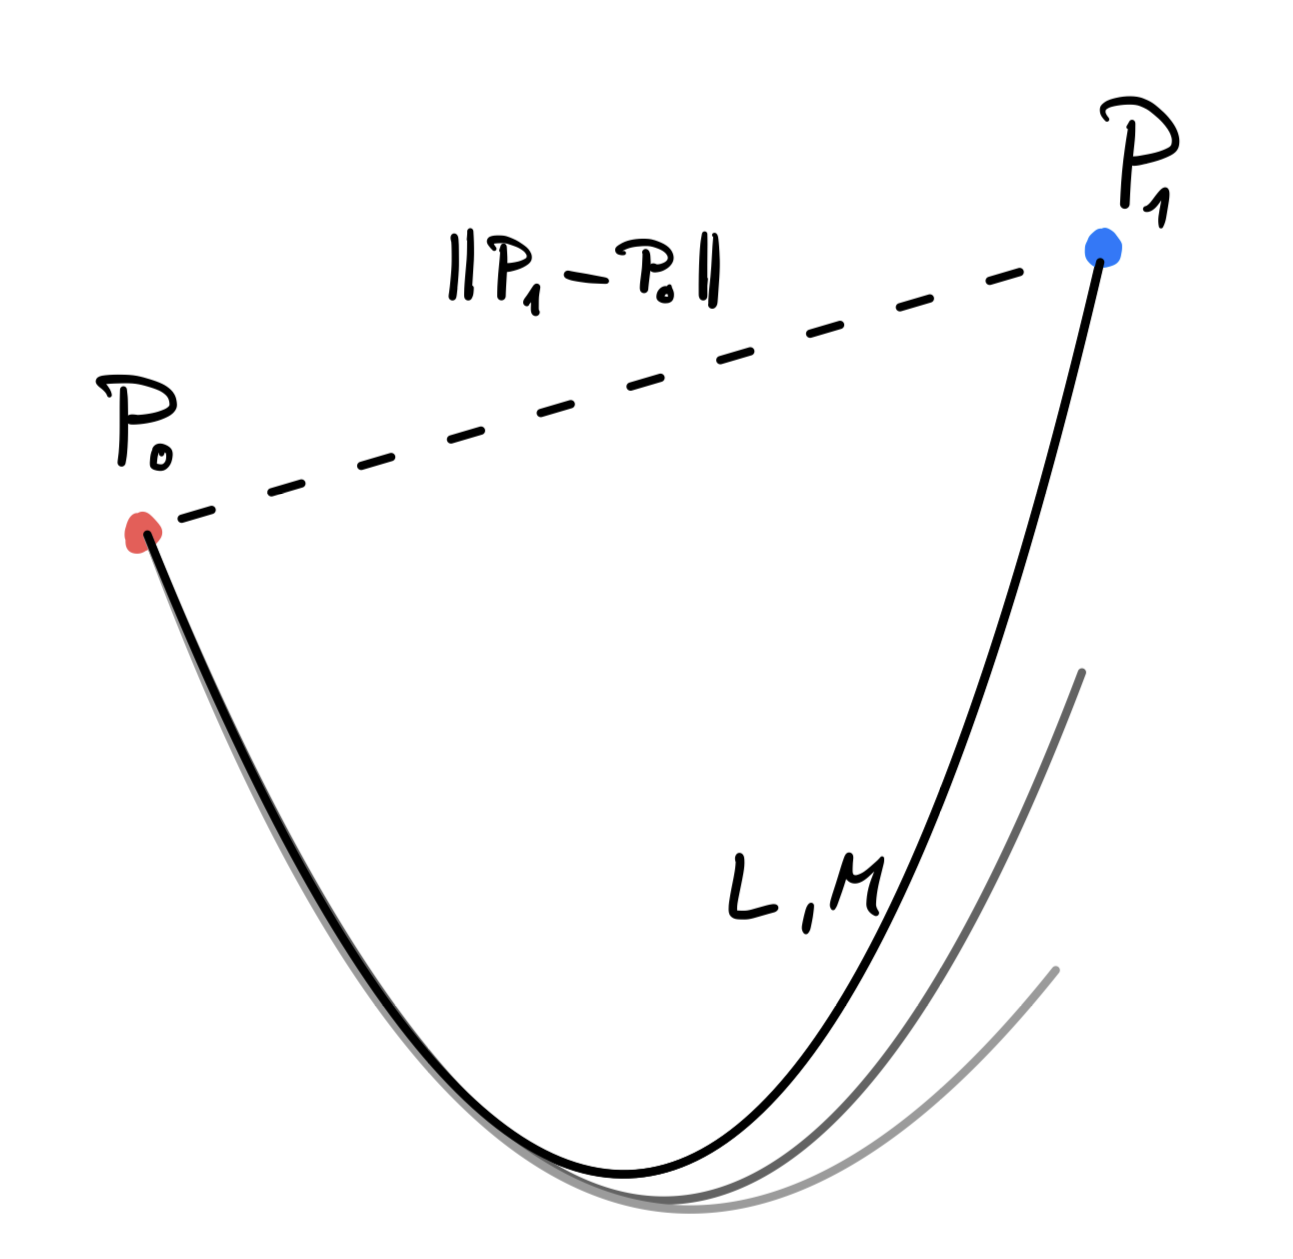
\includegraphics[width=0.45\textwidth]{slike/skica_uvod.png}
\caption{Skica problema z oznakami.}
\label{f:skica_uvod}
\end{figure}
Nalogo sem reševal v programskem jeziku Python z uporabo knjižnic Numpy, Scipy in Matplotlib.





\section{Izračun začetnega stanja}
Vrv ali veriga obešena na koncih, v mirujočem stanju visi v obliki verižnice. To je oblika črke 'U', ki se na prvi pogled zdi parabolična. Oblika te verižnice je odvisna od položaja sidrišč in porazdelitve mase po vrvi. V tem položaju ima vrv najmanjšo potencialno energijo. \par\vspace{5mm}

Začnemo z gibalnima enačbama za idealno gibkko vrv s predavanj
\begin{eqnarray}
\mu \frac{\pd^2 x}{\pd t^2} &=& \frac{\pd}{\pd s}\left(F(s)\frac{\pd x}{\pd s}\right) \\
\mu \frac{\pd^2 y}{\pd t^2} &=& \frac{\pd}{\pd s}\left(F(s)\frac{\pd y}{\pd s}\right) - \mu g,
\end{eqnarray}
kjer je $\mu = \frac{\diff m}{\diff s}$, $F(s)$ pa napetost v vrvi. Pri reševanju te naloge sem privzel, da je vrv homogena, torej $\mu = M/L$. Za stacionarno vrv vidimo, da je napetost v vodoravni smeri konstantna, napetost v navpični smeri pa je odvisna od dolžine vrvi od točke, kjer napetost opazujemo, do najnižje točke vrvi. \par\vspace{5mm}

Homogena viseča vrv zavzame obliko hiperboličnega cosinusa $y = a\cosh\left(\frac{x}{a}\right)$. Parameter $a$ sem numerično izračunal tako, da je energija minimalna, potem pa še premaknil krivuljo na pravo mesto, da povezuje levo in desno sidrišče. 

\begin{figure}[H]
\centering
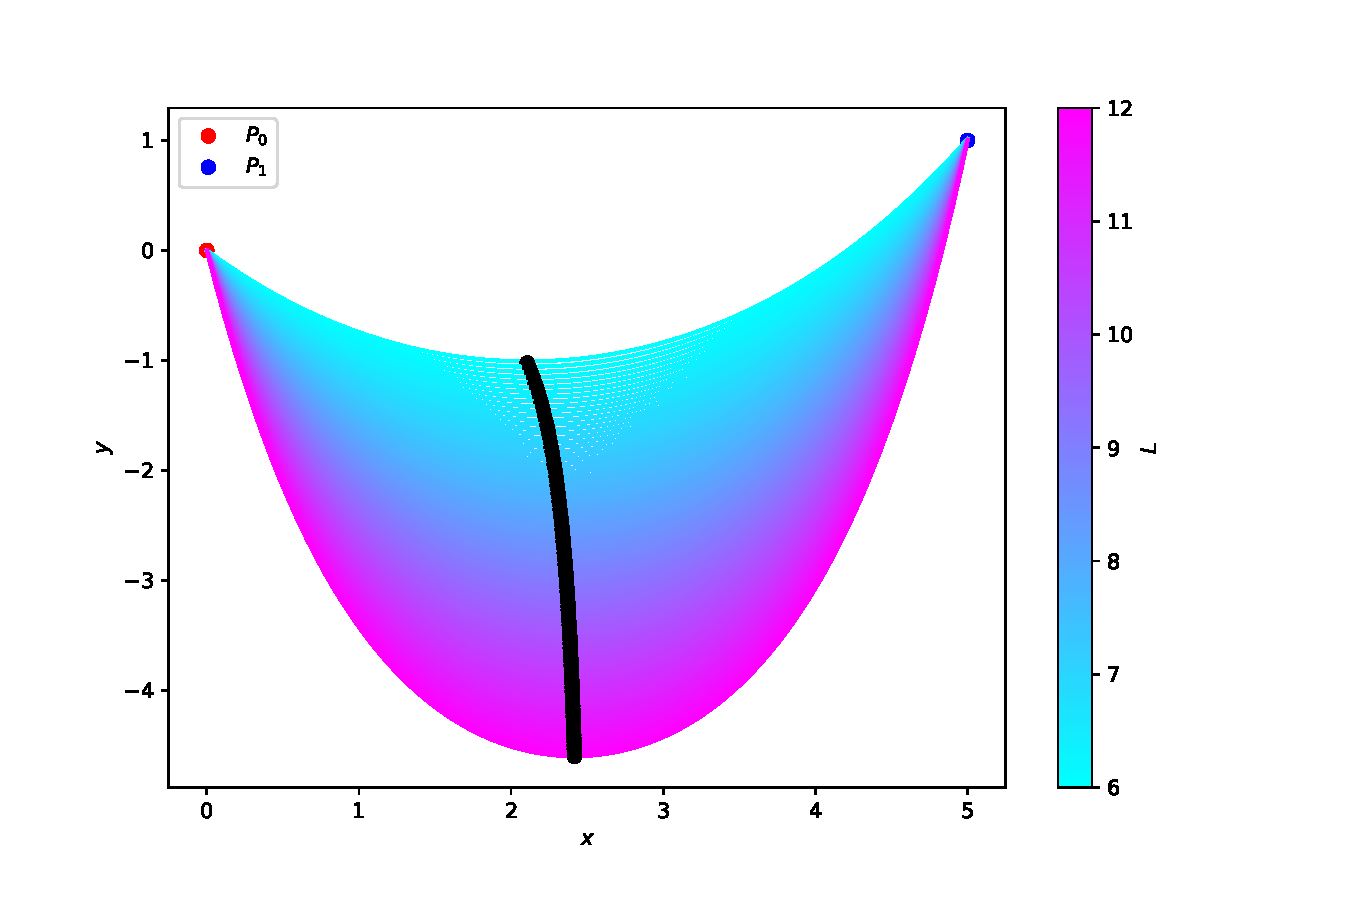
\includegraphics[width=0.75\textwidth]{grafi/catenary-L6.0-12.0-P00.0-0.0-P15.0-1.0.pdf}
\caption{Veriznica med točkama ${\bi P_0}(0, 0)$ in ${\bi P_1}(5, 1)$ za različne dolžine vrvi $L$. Rdeča in modra točka prikazujeta  ${\bi P_0}$ in ${\bi P_1}$, črne točke pa so najnižje točke krivulj. Barve krivulj prikazujejo različne dolžine vrvi od $L=6$ do $L=12$.}
\label{f:veriznice}
\end{figure}




\section{Diskretizacija vrvi}
Vrv ali verižico lahko diskretiziramo na različne načine. V tej nalogi bom vrv dolžine $L$ z maso $M$ razdelil na $n$ enako dolgih delov z maso $m=M/n$ in dolžino $l=L/n$. Ker so cevke toge, lahko opišemo obliko in položaj vrvi z $n$ spremenljivkami tako, da podamo kot vsakega delca vrvi glede na vodoravnico $\varphi_i$, $i = 1,..., n$. Kartezične  koordinate sredine vsakega segmenta potem lahko zapišemo kot
\begin{eqnarray}
x_i &=& \sum_{j=1}^{i-1}l\cos\varphi_j + \frac{1}{2}l\cos\varphi_i \\
y_i &=& \sum_{j=1}^{i-1}l\sin\varphi_j + \frac{1}{2}l\sin\varphi_i
\end{eqnarray}
Vsak segment ima vztrajnostni moment $J_i = \frac{1}{12} ml^2$. S tem znanjem lahko sestavimo kinetično in potencialno energijo vrvi
\begin{eqnarray}
T &=& \frac{1}{2}\sum_{i=1}^n \left[m(\dot{x}^2 + \dot{y}^2) + J_i\dot{\varphi_i}^2 \right], \\
V &=& \sum_{i=1}^n mgy_i.
\end{eqnarray}
Energiji izrazimo s koti $\varphi_i$ \cite{simplechainfall}
\begin{eqnarray}
T &=& ml^2\sum_{i=1}^n\left[\frac{1}{2}(n-i) + \frac{1}{6}\right]\dot{\varphi}_i^2 + ml^2\sum_{i=1}^n\sum_{j = i+1}^n \left[ n-j + \frac{1}{2} \right]\dot{\varphi}_i\dot{\varphi}_j\cos(\varphi_i - \varphi_j)	\\
V &=& \sum_{i=1}^n\left(n-i + \frac{1}{2}\right)mgl\sin\varphi_i
\end{eqnarray}
in zapišemo Lagrangian tega sistema $\Lag = T - V$. Dobimo sistem Euler-Lagrangeovih enačb
\begin{equation}
\frac{\diff }{\diff t}\left(\frac{\pd\Lag}{\pd\dot{\varphi}_i}\right) - \frac{\pd\Lag}{\pd\varphi}_i = 0, \qquad i=1,...,n
\end{equation}
in ga prepišemo kot
\begin{equation}
\sum_{j=1}^n m_{ij}c_{ij}\ddot{\varphi}_j + \sum_{j=1}^n m_{ij}s_{ij}\dot{\varphi}_j^2 + \frac{g}{l}q_ic_i = 0, \qquad i=1,...,n.
\label{eq:el-ketna-osn}
\end{equation}
V tem sistemu enačb je $c_{ij} = \cos(\varphi_i-\varphi_j)$, $s_{ij} = \sin(\varphi_i-\varphi_j)$, $c_i=\cos\varphi_i$, $q_i = n-i+\frac{1}{2}$. Matriko faktorjev $m_{ij}$ pa izračunamo kot $m_{ii} = n-i+1/3$ za $i=j$ in $m_{ij}=n-\mathrm{max}(i, j) +1/2$, ko $i\neq j$ \cite{simplechainfall}. Izrazimo $\ddot{\varphi}_i$ in numerično rešimo sistem diferencialnih enačb. Uporabil sem metodo Runge-Kutta četrtega reda. Za testni primer sem uporabljal vodoravno raztegnjeno vrv.





\section{Padanje vodoravno raztegnjene vrvi}
Levi konec vrvi ostane pritejen in se ne premika, desni konec pa spustimo in zaradi gravitacijske sile začne padati. Kot je vidno na sliki \ref{f:padanje-zac}, desni konec vrvi začne padati skoraj v vodoravni obliki, na levi strani pa vidimo vedno strmejšo premico. To je pravilno obnašanje za tako vrv. Težave se pojavijo, ko vrv preide preko raztegnjene lege in prehaja v obliko črke J. Pri izhodišču se $"$zmečka$"$, proti koncu pa se tudi začne nenavadno lomiti. Mogoče je tako obnašanje lahko opaženo v verigi, za vrv pa je nenaravno.

\begin{figure}[H]
\centering
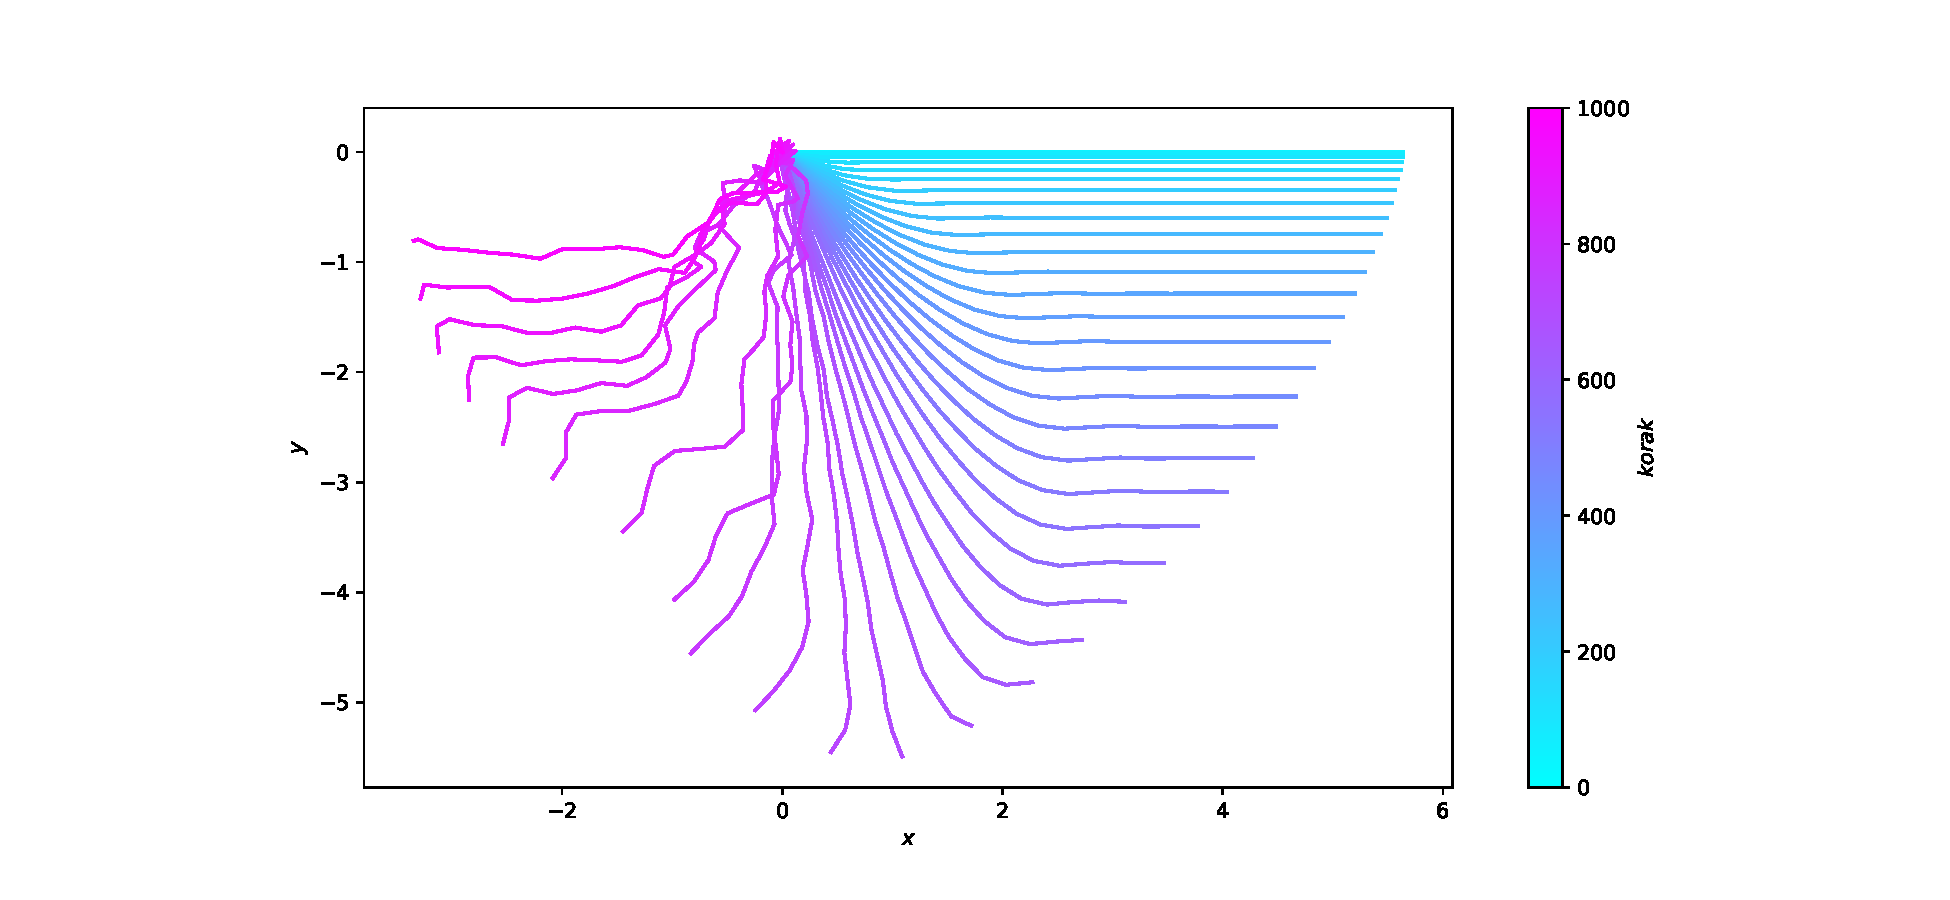
\includegraphics[width=0.95\textwidth]{grafi/padvrv-n25-l0.24-dt0.01-t10.0-freq25.pdf}
\caption{Potek padanja verižice s 25 členi iz vodoravne pozicije po enačbi \eqref{eq:el-ketna-osn}. Barve prikazujejo časovni potek integracije. Verižica začne v svetlo modrem položaju, konča pa v roza barvi. Prikazan je vsak 25. korak. Ostali parametri: $m=0.2$, $g=1$.}
\label{f:padanje-zac}
\end{figure}

Enačba \eqref{eq:el-ketna-osn} ne upošteva vpliva sosednjih členov na gibanje. V primeru vrvi se gibanje dveh sosednjih segmentov ne more poljubno razlikovati. To lahko upoštevamo tako, da v sistem vpeljemo dušenje preko Rayleighove disipacijske funkcije \cite{tomazevski}
\begin{equation}
\mathcal{R} = \frac{1}{2}r\sum_{i=1}^n\left(\dot{\varphi}_i - \dot{\varphi}_{i-1}\right)^2.
\end{equation}
Posodobimo še sistem Euler-Lagrangeovih enačb
\begin{eqnarray}
\frac{\diff }{\diff t}\left(\frac{\pd\Lag}{\pd\dot{\varphi}_i}\right) - \frac{\pd\Lag}{\pd\varphi}_i + \frac{\pd\mathcal{R}}{\pd\dot{\varphi}_i}&=& 0 \\
\sum_{j=1}^n m_{ij}c_{ij}\ddot{\varphi}_j + \sum_{j=1}^n m_{ij}s_{ij}\dot{\varphi}_j^2 + \frac{g}{l}q_ic_i + \frac{r}{ml^2} \left(\dot{\varphi}_{i+1} - 2\dot{\varphi}_i + \dot{\varphi}_{i-1} \right) &=& 0,
\label{eq:el-final}
\end{eqnarray}
kjer je $m$ masa člena verige z dolžino $l$ in $r$ poljuben parameter, ki določa kako močno bo dušenje. Enačbo \eqref{eq:el-final} podobno kot prej rešimo z numerično metodo Runge-Kutta četrtega reda. Parameter $r$ sem nastavil na najmanjšo vrednost, da se vrv ni več lomila. To sem našel nekje pri $r\in[0.0005, 0.001]$.

\begin{figure}[H]
\centering
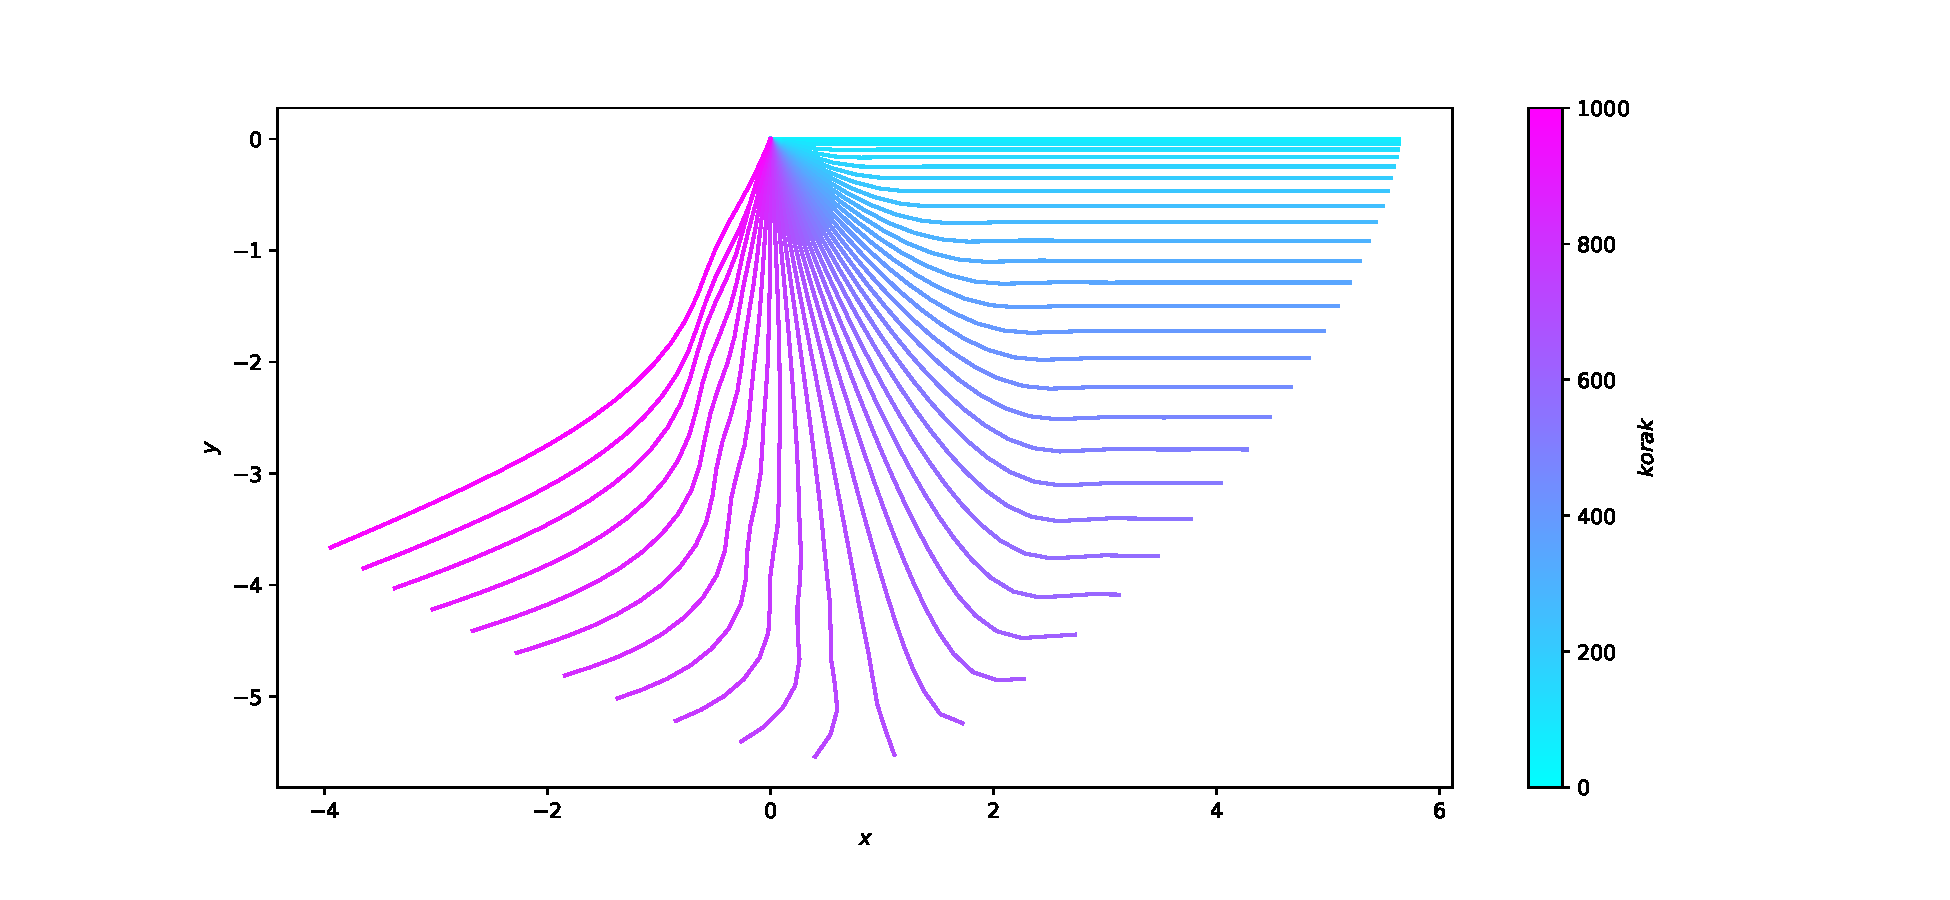
\includegraphics[width=0.95\textwidth]{grafi/padvrv-popR-n25-l0.24-m0.2-r0.001-dt0.01-t10.0-freq25.pdf}
\caption{Potek padanja verižice s 25 členi iz vodoravne pozicije po enačbi \eqref{eq:el-final} pri $r=0.001$. Prikazan je vsak 25. korak. Ostali parametri: $m=0.2$, $g=1$.}
\label{f:padanje-r}
\end{figure}

Na sliki \ref{f:padanje-r} vidimo, da veriga na začetku pada enako kot prej (slika \ref{f:padanje-zac}), v levem delu slike pa je obnašanje je bolj podobno pričakovanemu obnašanju vrvi. Pri tem je pomembno preveriti, če se po dolgem času viseča vrv izniha, kar je prikazano na sliki \ref{f:padanje-izniha}.

\begin{figure}[H]
\centering
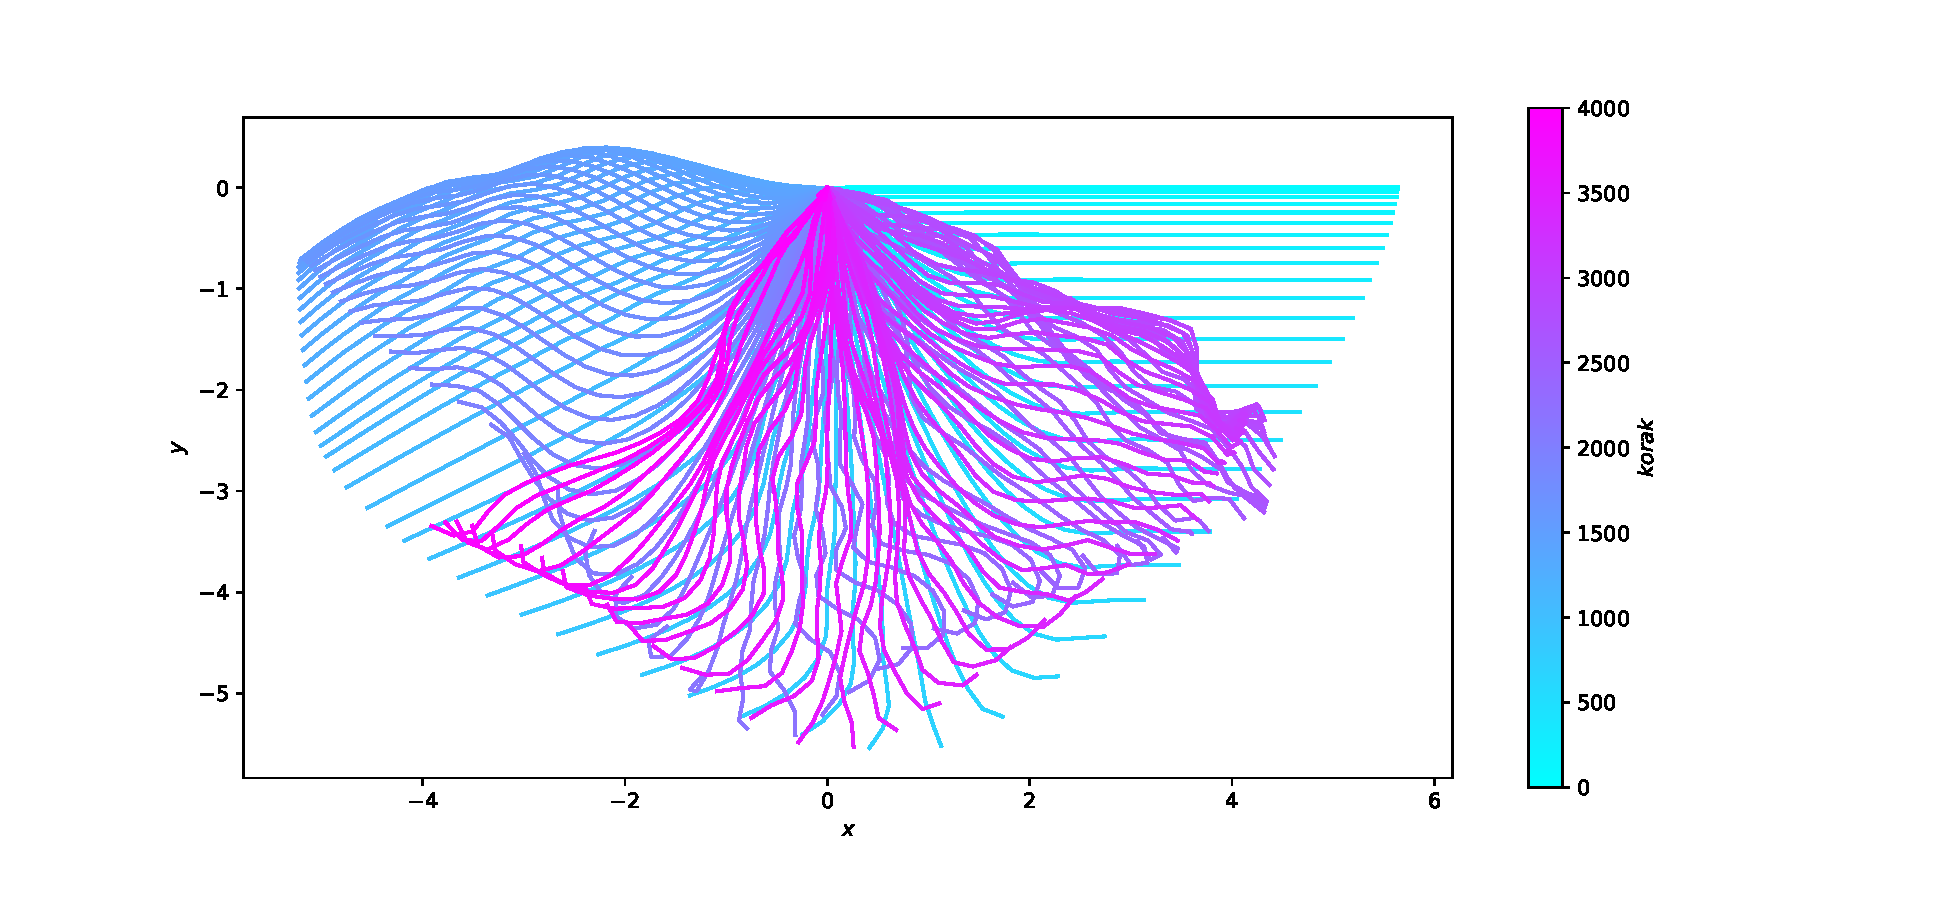
\includegraphics[width=0.95\textwidth]{grafi/padvrv-popR-n25-l0.24-m0.2-dt0.01-t10.0-freq25.pdf}
\caption{Potek padanja verižice s 25 členi iz vodoravne pozicije po enačbi \eqref{eq:el-final} pri $r=0.001$. Prikazan je vsak 25. korak. Ostali parametri: $m=0.2$, $g=1$.}
\label{f:padanje-izniha}
\end{figure}





\section{Padanje verižnice}
Poglejmo si še, kako pada vrv ali veriga, če na začetku visi v obliki verižnice (slika \ref{f:padanje-cat}). Vidimo da, podobno kot prej, desni del približno ohranja začetno obliko in se spušča. Opazna razlika pa je, da se vrv prej začne kriviti v nasprotno smer (v obliko črke J) kot pa se je pri spustu iz raztegnjenega položaja.

\begin{figure}[H]
\centering
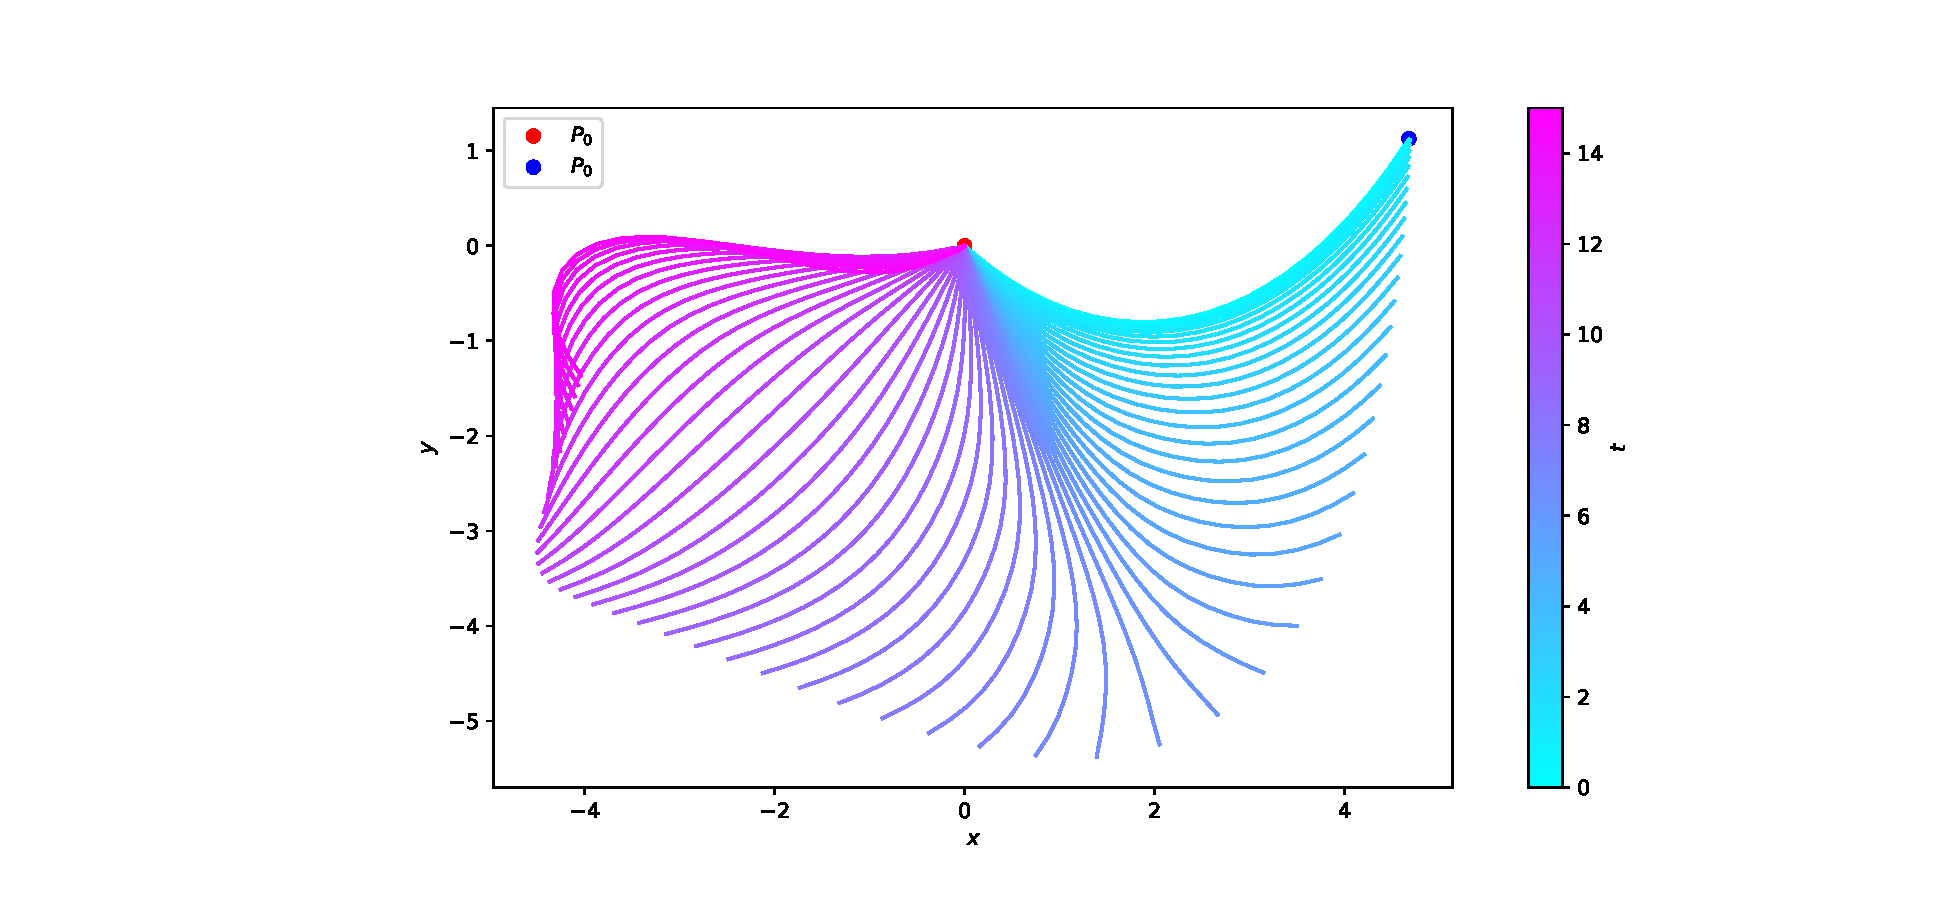
\includegraphics[width=0.95\textwidth]{grafi/falling_chain_P.5-1_L.6_n.25_t.15_r.0.001_m.0.2_g.1_dt.0.010006671114076937_freq.25.pdf}
\caption{Potek padanja verižice dolžine $L=6$ s 25 členi, ki povezuje točki ${\bi P_0}(0, 0)$ in ${\bi P_1}(5, 1)$. Parametri pa so nastavljeni kot $r=0.001$, $m=0.2$, $g=1$. Časovni korak integracije je enak $\diff t = 0.01$.}
\label{f:padanje-cat}
\end{figure}





\subsection{Odvisnost od horizontalne razdalje med sidriščema}
Poglejmo si še, kaj se dogaja, ko premikamo desno sidrišče ${\bi P_1}$. Obravnaval bom primere, ko sta sidrišči na isti višini in spreminjal horizontalno razdaljo $d$ med njima. Izbral sem štiri testne primere za $d=1, 3, 5, 6$, pri dolžini vrvi $L = 6$, in potek padanja prikazal na sliki \ref{f:horizontalno}.


\begin{figure}[H]
\centering
\begin{subfigure}{0.297\textwidth}
	\centering
	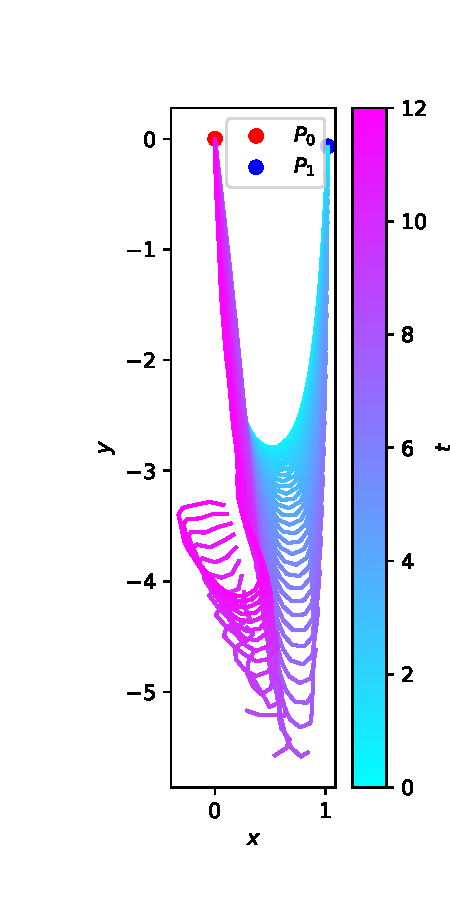
\includegraphics[width=0.95\textwidth]{grafi/falling_chain_P.1.0--0.2_L.6_n.47_t.12_r.0.0005_m.0.2_g.1_dt.0.01_freq.25.pdf}
	\caption{$d = 1$.}
	\label{f:hor-1}
\end{subfigure}
\begin{subfigure}{0.693\textwidth}
	\centering
	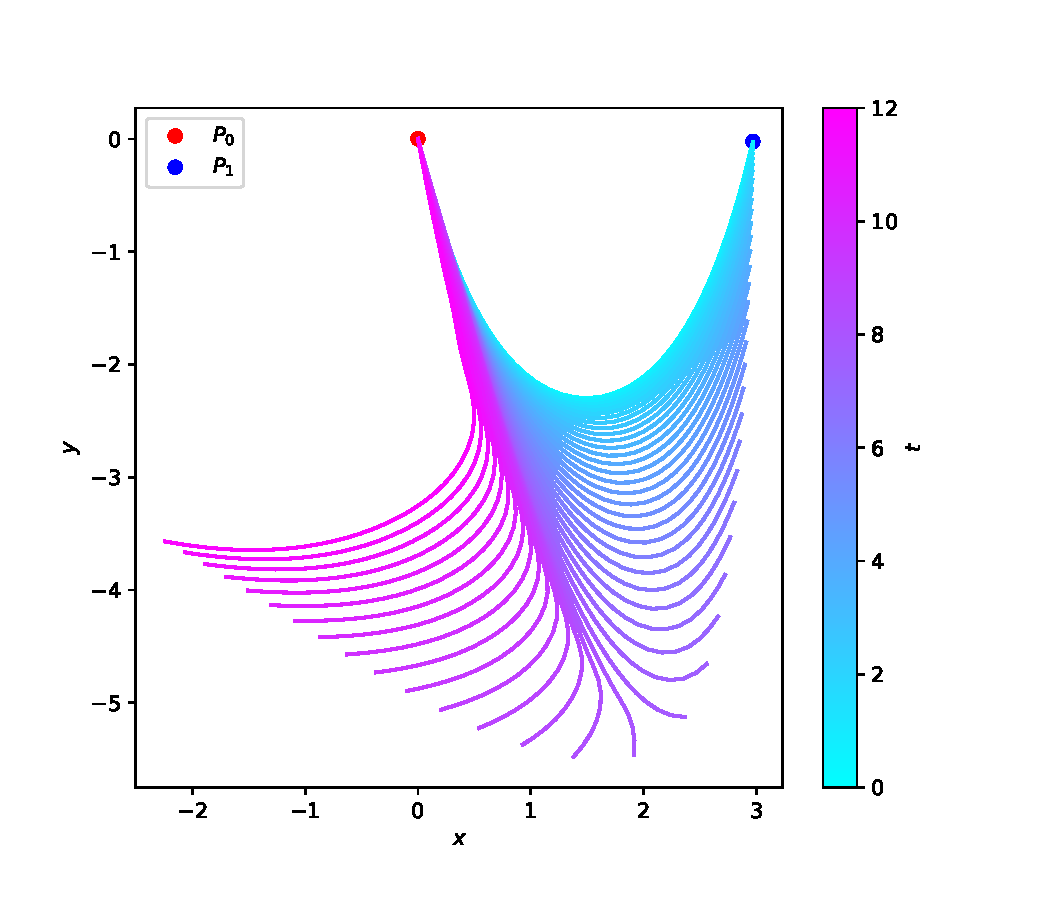
\includegraphics[width=0.95\textwidth]{grafi/falling_chain_P.3.0--0.15_L.6_n.48_t.12_r.0.0005_m.0.2_g.1_dt.0.01_freq.25.pdf}
	\caption{$d = 3$.}
	\label{f:hor-3}
\end{subfigure}
\end{figure}
\begin{figure}[H]\ContinuedFloat
\begin{subfigure}{0.495\textwidth}
	\centering
	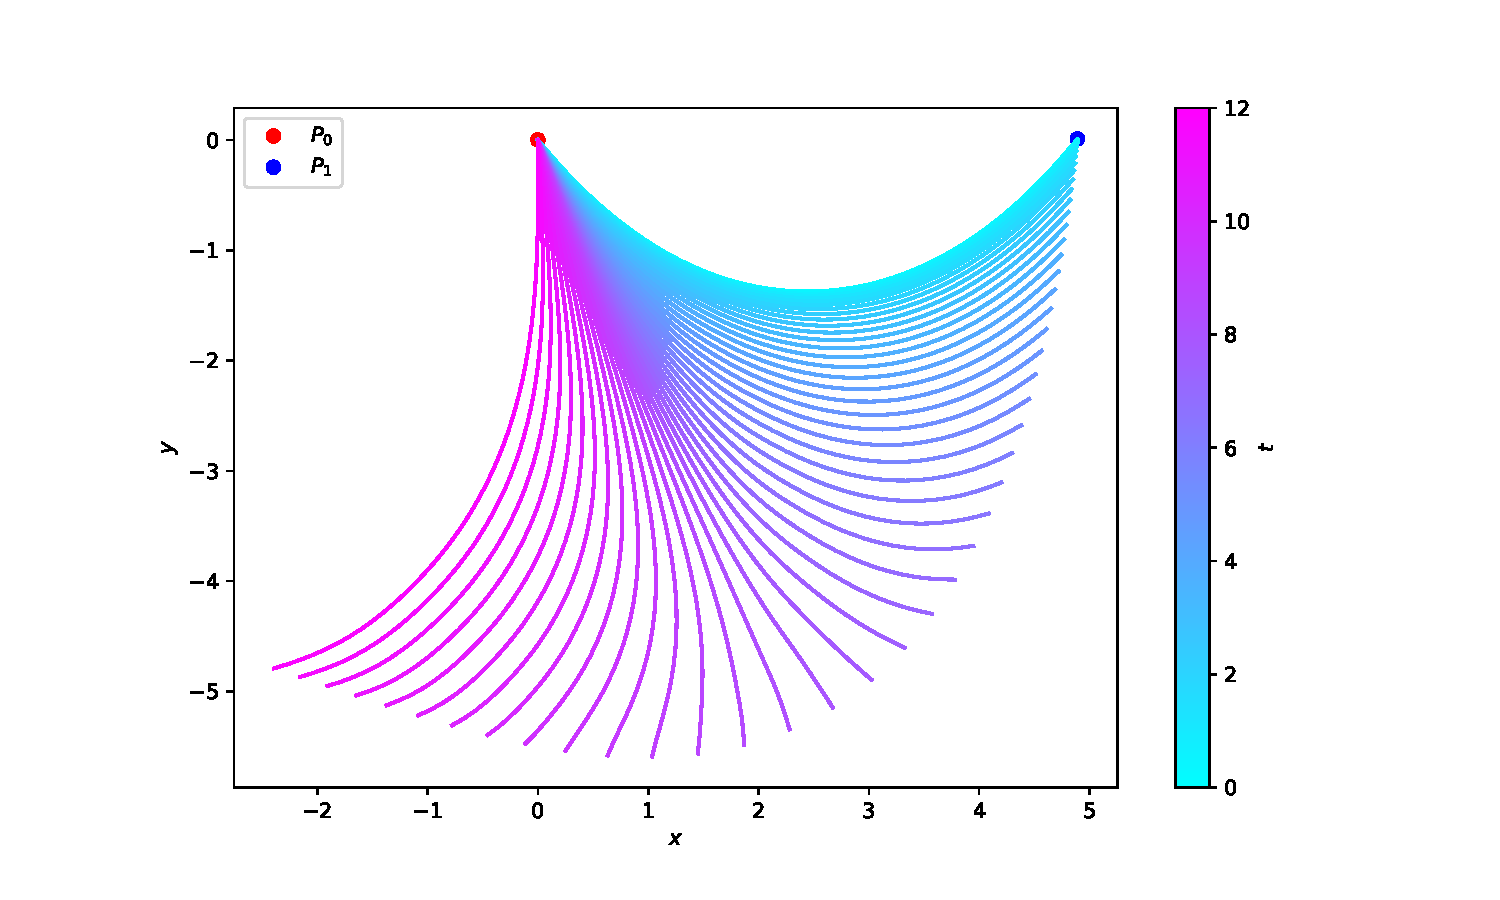
\includegraphics[width=0.95\textwidth]{grafi/falling_chain_P.5.0--0.05_L.6_n.48_t.12_r.0.0005_m.0.2_g.1_dt.0.01_freq.25.pdf}
	\caption{$d = 5$.}
	\label{f:hor-5}
\end{subfigure}
\begin{subfigure}{0.495\textwidth}
	\centering
	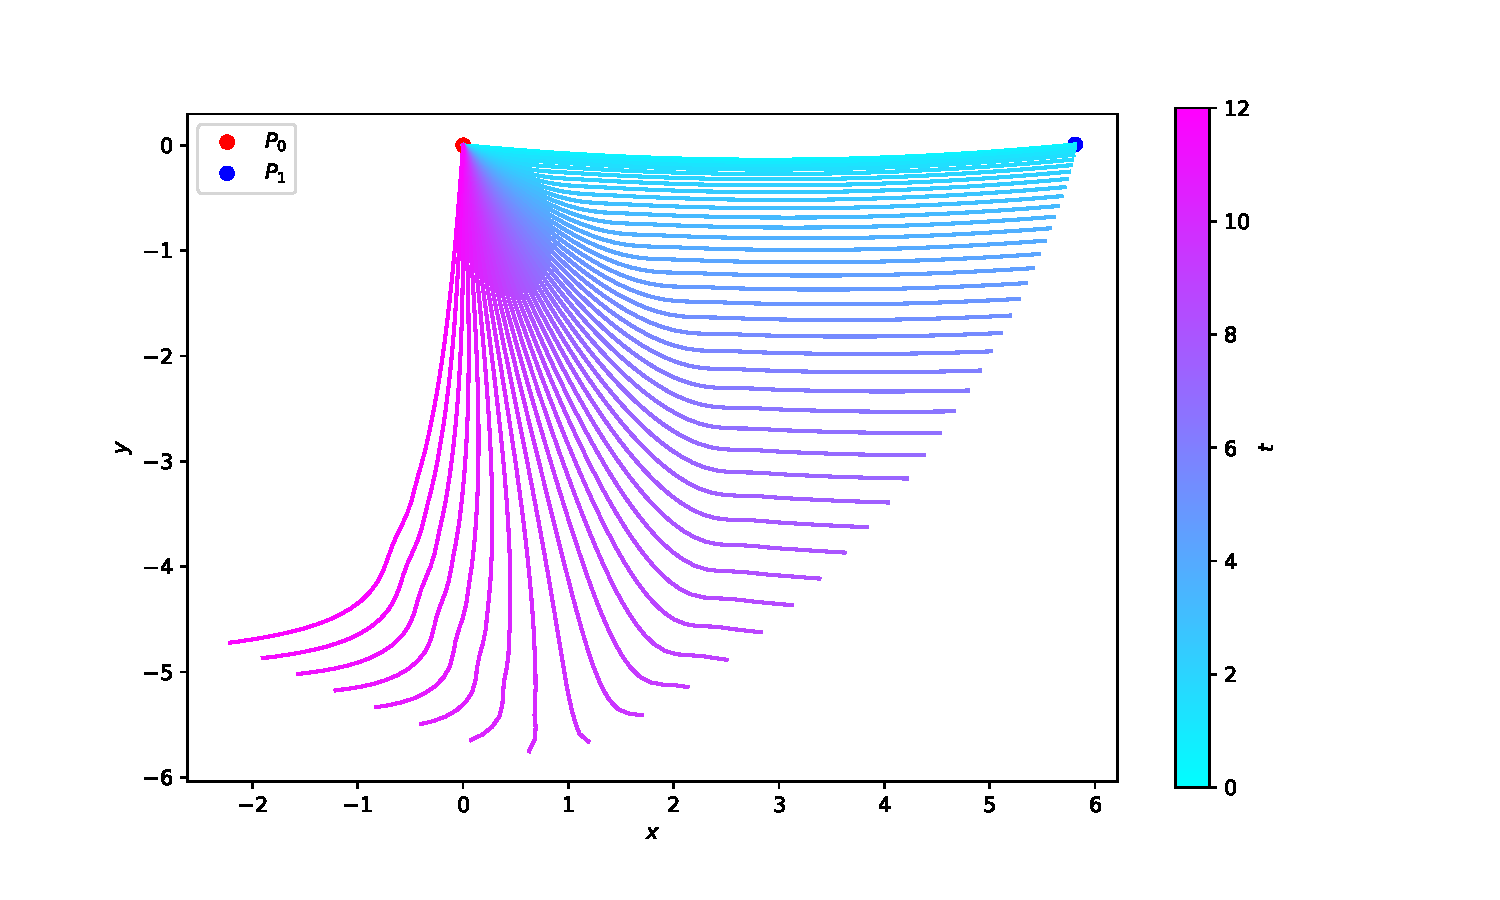
\includegraphics[width=0.95\textwidth]{grafi/falling_chain_P.5.99-0.0_L.6_n.50_t.12_r.0.0005_m.0.2_g.1_dt.0.01_freq.25.pdf}
	\caption{$d = 6$.}
	\label{f:hor-6}
\end{subfigure}
\caption{Padanje vrvi dolžine $L=6$ pri različnih oddaljenostih sidrišč $d$. Parametri pa so nastavljeni na $r=0.0005$, $m=0.2$, $g=1$. Časovni korak integracije je enak $\diff t = 0.01$. Verigo sestavlja $n=50$ členov.}
\label{f:horizontalno}
\end{figure}


Opazimo, da se vrv ali veriga med padanjem ne glede na oddaljenost sidrišč zvija v podobne oblike. Boljši vpogled v gibanje nam da primerjava hitrosti koncev vrvi, ki je prikazana na sliki \ref{f:horizontalno-hitrosti}. Največje izstopanje opazimo na sliki \ref{f:hor-1}, kjer $d=1$. Tam vrv po padcu ne zaniha lepo ampak se močneje zakrivi. To sunkovito gibanje je lepo opazno na faznem diagramu (slika \ref{f:hor-v-fd}), kjer svetlo modra krivulja postane zelo groba. \par\vspace{5mm}


Na začetku z naraščanjem razdalje $d$ maksimalna hitrost pada in konec vrvi najvišjo hitrost doseže prej. Zelo zanmivo pa je, da maksimalna hitrost pri raztegnjeni vrvi $d=6$ spet naraste in je dosežena še kasneje. Grafa hitrosti za $d=1$ in $d=6$ na sliki \ref{f:hor-v} ostala brez vrhov, verjetno zaradi omejenosti numerične metode.


\begin{figure}[H]
\centering
\begin{subfigure}{0.495\textwidth}
	\centering
	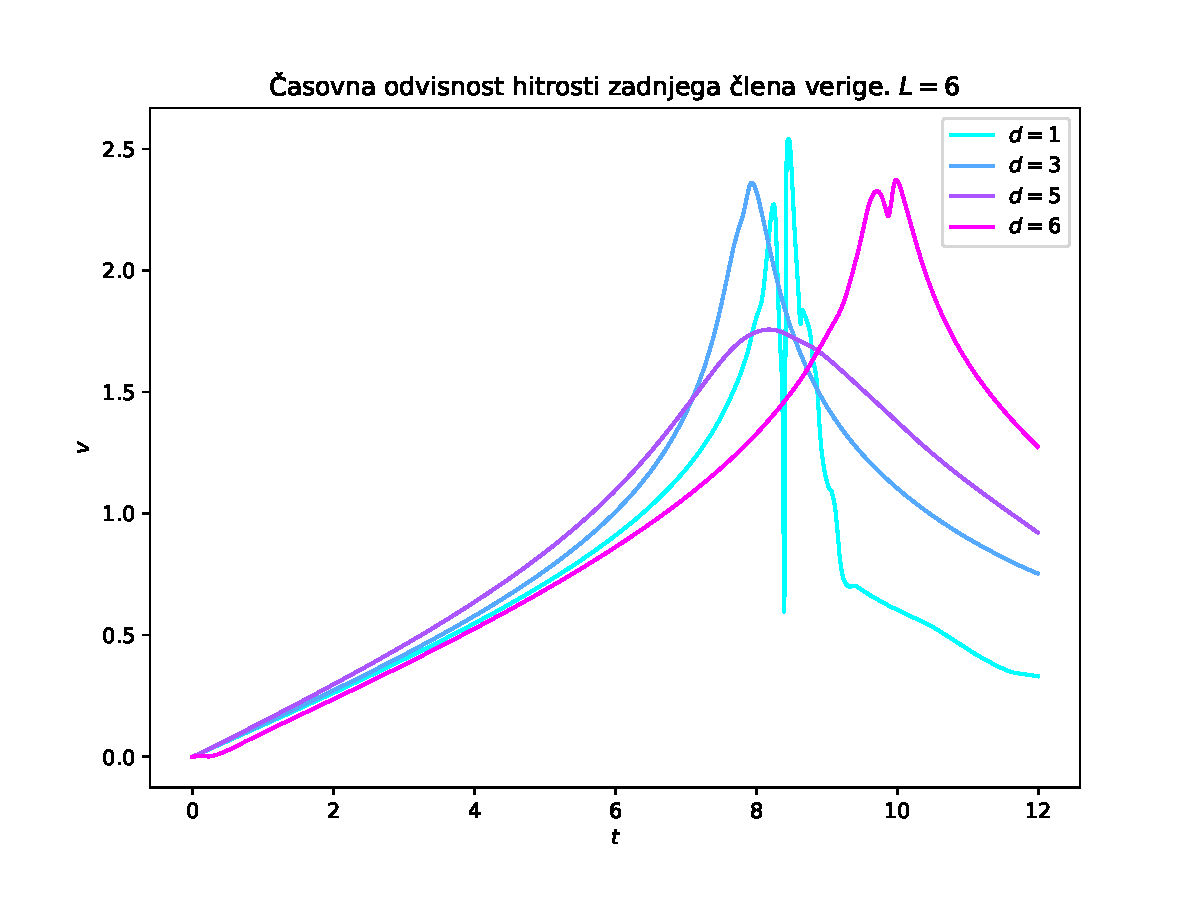
\includegraphics[width=0.95\textwidth]{grafi/hitrost_siroko.pdf}
	\caption{Časovna odvisnost absolutne hitrosti.}
	\label{f:hor-v}
\end{subfigure}
\begin{subfigure}{0.495\textwidth}
	\centering
	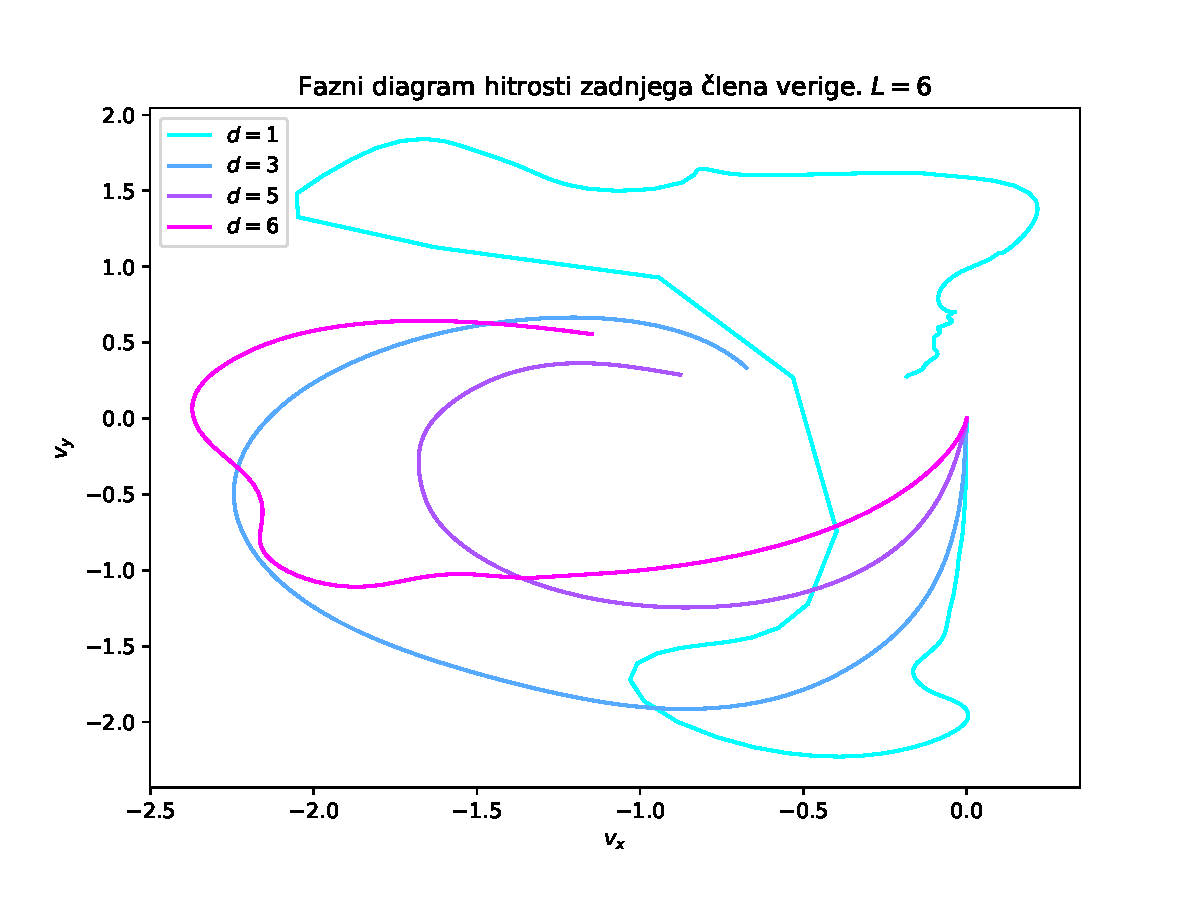
\includegraphics[width=0.95\textwidth]{grafi/hitrost_siroko_xy.pdf}
	\caption{Fazni diagram hitrosti.}
	\label{f:hor-v-fd}
\end{subfigure}
\caption{Hitrost konca vrvi dolžine $L=6$ pri padanju iz različno oddaljenih sidrišč $d$. Parametri pa so nastavljeni na $r=0.0005$, $m=0.2$, $g=1$. Časovni korak integracije je enak $\diff t = 0.01$. Verigo sestavlja $n=50$ členov.}
\label{f:horizontalno-hitrosti}
\end{figure}




Zanimivo bi bilo tudi raziskati odvisnost maksimalne hitrosti od horizonatalne razdalje med sidriščima $d$. Zato sem spet za vrvi dolžine $L=6$ razdeljene na 50 segmentov izračunal maksimalne hitrosti prostega konca vrvi. Ker je izračun numerično zelo zahteven sem izbral samo 14 različnih razdalj. Odvisnost je lepo vidna na sliki \ref{f:vmax}. Na začetku hitrost malo naraste, potem pa pada dokler $d\approx 80\% L$, kjer pa spet začne naraščati.

\begin{figure}[H]
\centering
\includegraphics[width=0.7\textwidth]{grafi/vmax_od_d_s-1.5789473684210527_f-6.0_k-14.pdf}
\caption{Odvisnost najvišje hitrosti konca vrvi $v_{\rm{max}}$ od razmaka sidrišč $d$. Parametri pa so nastavljeni na $r=0.0005$, $m=0.2$, $g=1$. Časovni korak integracije je enak $\diff t = 0.01$. Verigo sestavlja $n=50$ členov.}
\label{f:vmax}
\end{figure}





\subsection{Odvisnost od vertikalnega razmika sidrišč}
Poglejmo še, kaj se dogaja, ko spreminjamo višino $h$ med točkama ${\bi P_0}$ in ${\bi P_1}$. Kot prej bom premikal samo ${\bi P_1}$ med višinami $h = -2, 0, 2, 4$, horizontalna oddaljenost pa bo kostantna $d=3$. Vrv je dolga $L=6$ in razdeljena na 50 členov. Potek padanja vrvi sem za vsakega od teh primerov narisal na sliki \ref{f:vertikalno}. Tokrat so razlike med oblikami bolj opazne.



\begin{figure}[H]
\centering
\begin{subfigure}{0.475\textwidth}
	\centering
	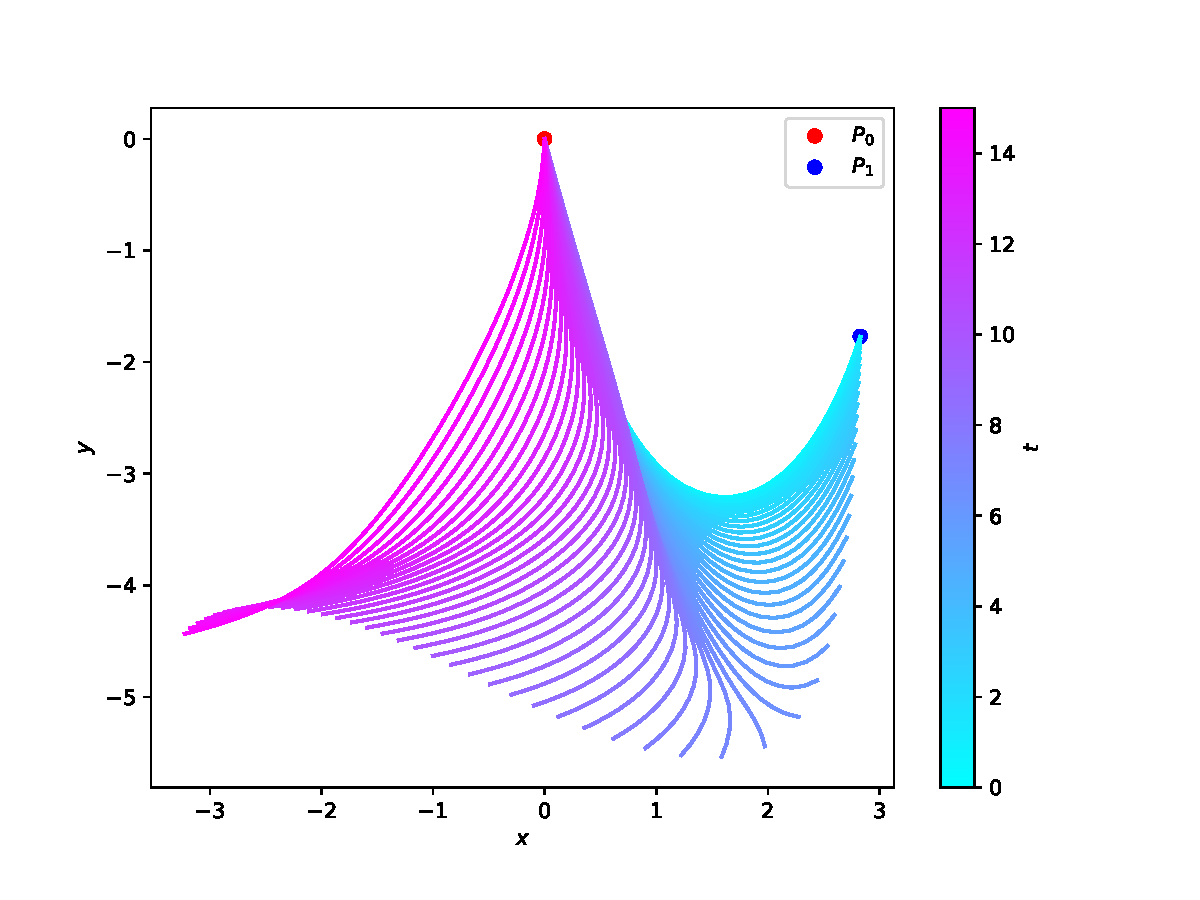
\includegraphics[width=0.95\textwidth]{grafi/falling_chain_P.3.0--2.0_L.6_n.50_t.15_r.0.0005_m.0.2_g.1_dt.0.01_freq.25.pdf}
	\caption{$h = -2$.}
	\label{f:ver--2}
\end{subfigure}
\begin{subfigure}{0.515\textwidth}
	\centering
	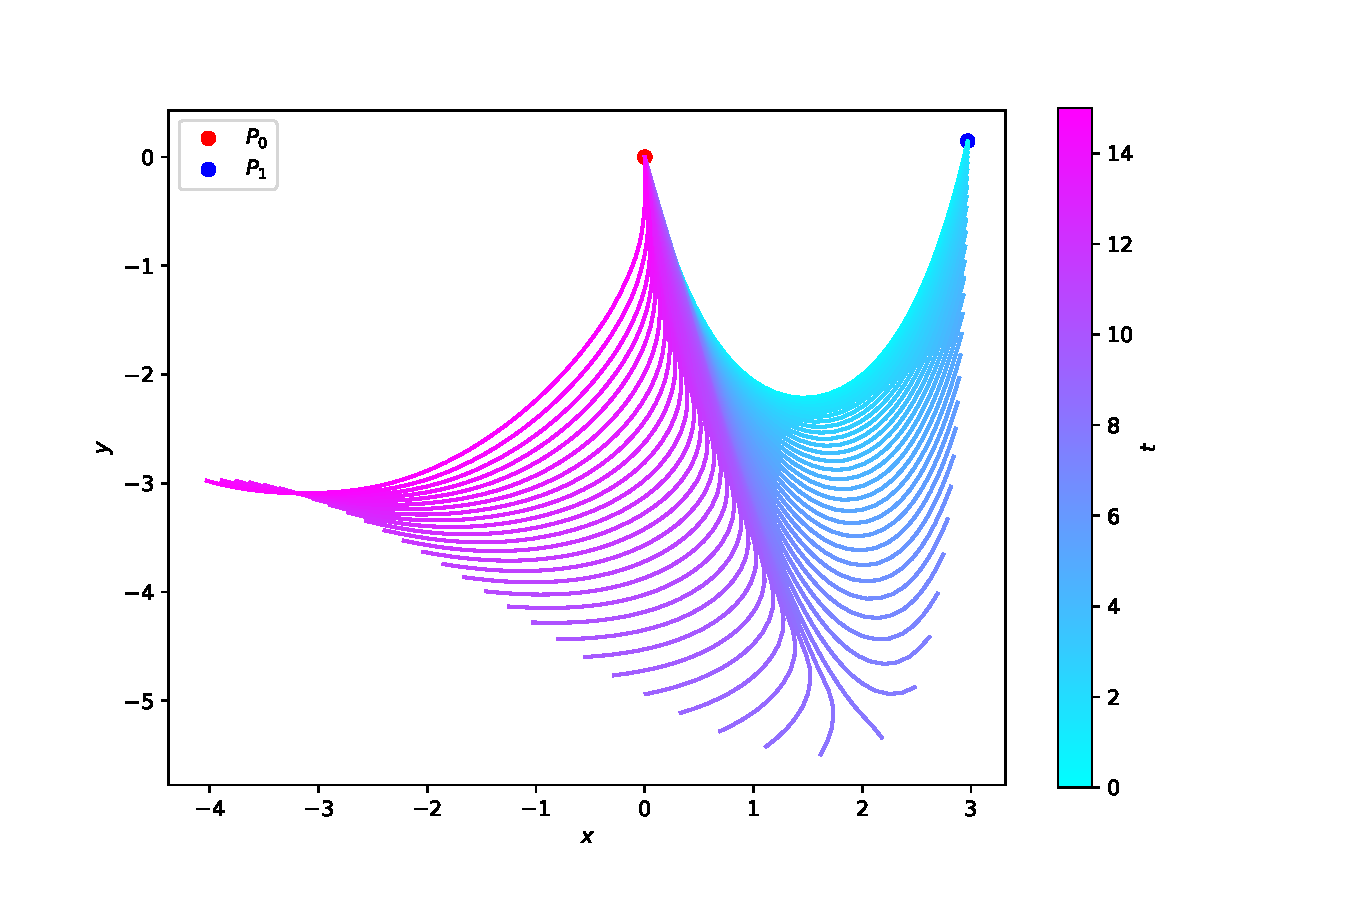
\includegraphics[width=0.95\textwidth]{grafi/falling_chain_P.3.0-0.0_L.6_n.48_t.15_r.0.0005_m.0.2_g.1_dt.0.01_freq.25.pdf}
	\caption{$h = 0$.}
	\label{f:ver-0}
\end{subfigure}
\end{figure}
\begin{figure}[H]\ContinuedFloat
\begin{subfigure}{0.575\textwidth}
	\centering
	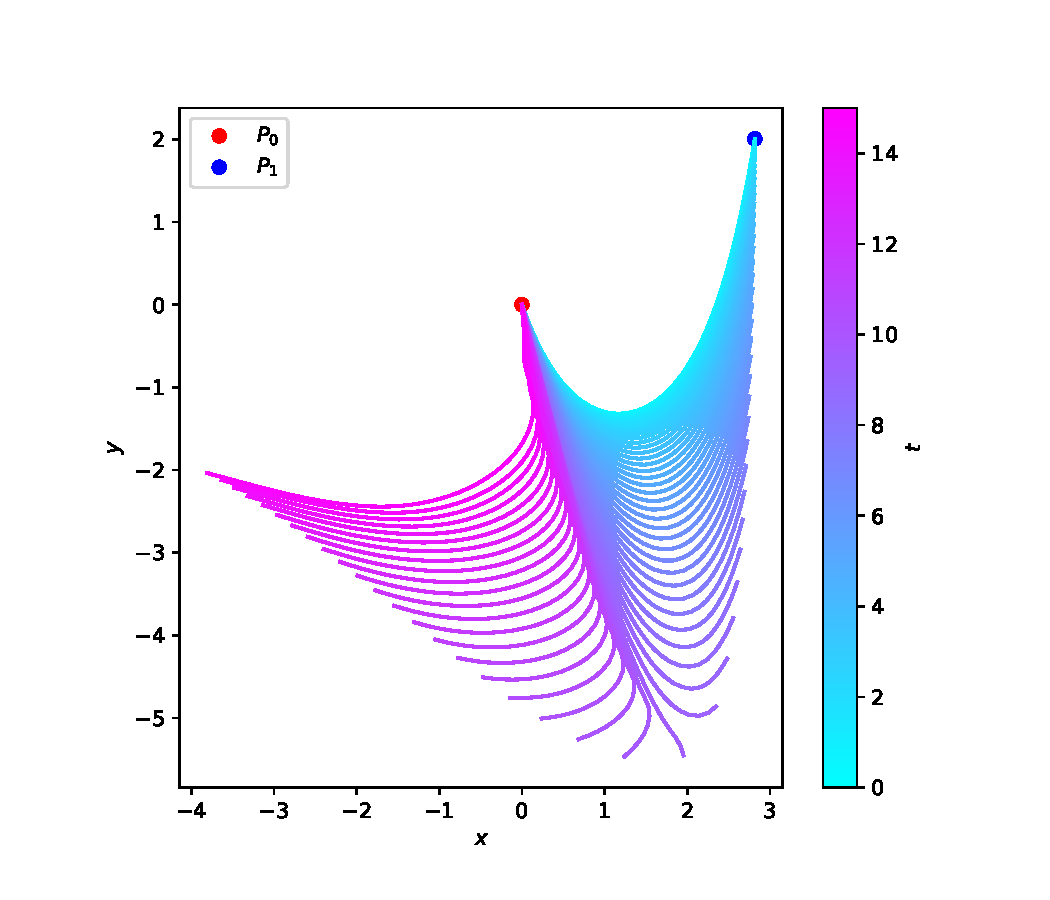
\includegraphics[width=0.95\textwidth]{grafi/falling_chain_P.3.0-2.0_L.6_n.50_t.15_r.0.0005_m.0.2_g.1_dt.0.01_freq.25.pdf}
	\caption{$h = 2$.}
	\label{f:ver-2}
\end{subfigure}
\begin{subfigure}{0.415\textwidth}
	\centering
	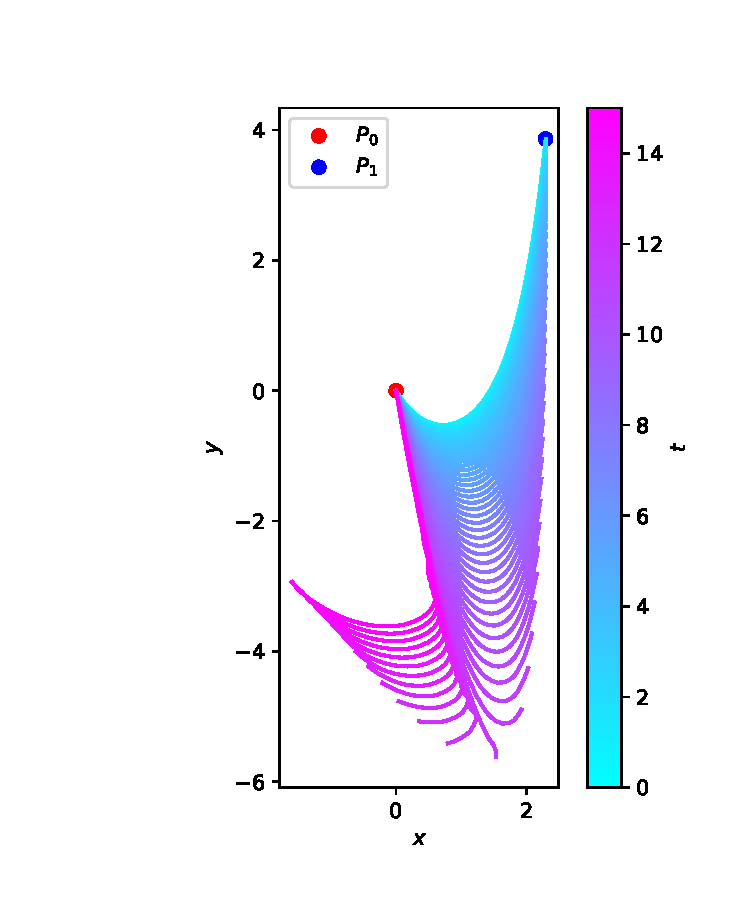
\includegraphics[width=0.95\textwidth]{grafi/falling_chain_P.3.0-4.0_L.6_n.60_t.15_r.0.0005_m.0.2_g.1_dt.0.01_freq.25.pdf}
	\caption{$h = 4$.}
	\label{f:ver-4}
\end{subfigure}
\caption{Padanje vrvi dolžine $L=6$ pri različnih višinskih razlikah med sidriščema $h$. Parametri pa so nastavljeni na $r=0.0005$, $m=0.2$, $g=1$. Časovni korak integracije je enak $\diff t = 0.01$. Verigo sestavlja $n=50$ členov.}
\label{f:vertikalno}
\end{figure}

Spet je vredno pogledati, kaj se dogaja s hitrostjo spuščenega konca vrvi. Na sliki \ref{f:vertikalno-hitrosti} sta prikazana časovna odvisnost in histogram hitrosti zadnjega člena za vse štiri primere. Na sliki \ref{f:ver-v} lahko vidimo, da z naraščanjem višine hitrost narašča, konec vrvi pa jo doseže vedno kasneje. Oboje je veliko jasneje vidno kot pri primeru različnih horizontalnih razdalj.


\begin{figure}[H]
\centering
\begin{subfigure}{0.495\textwidth}
	\centering
	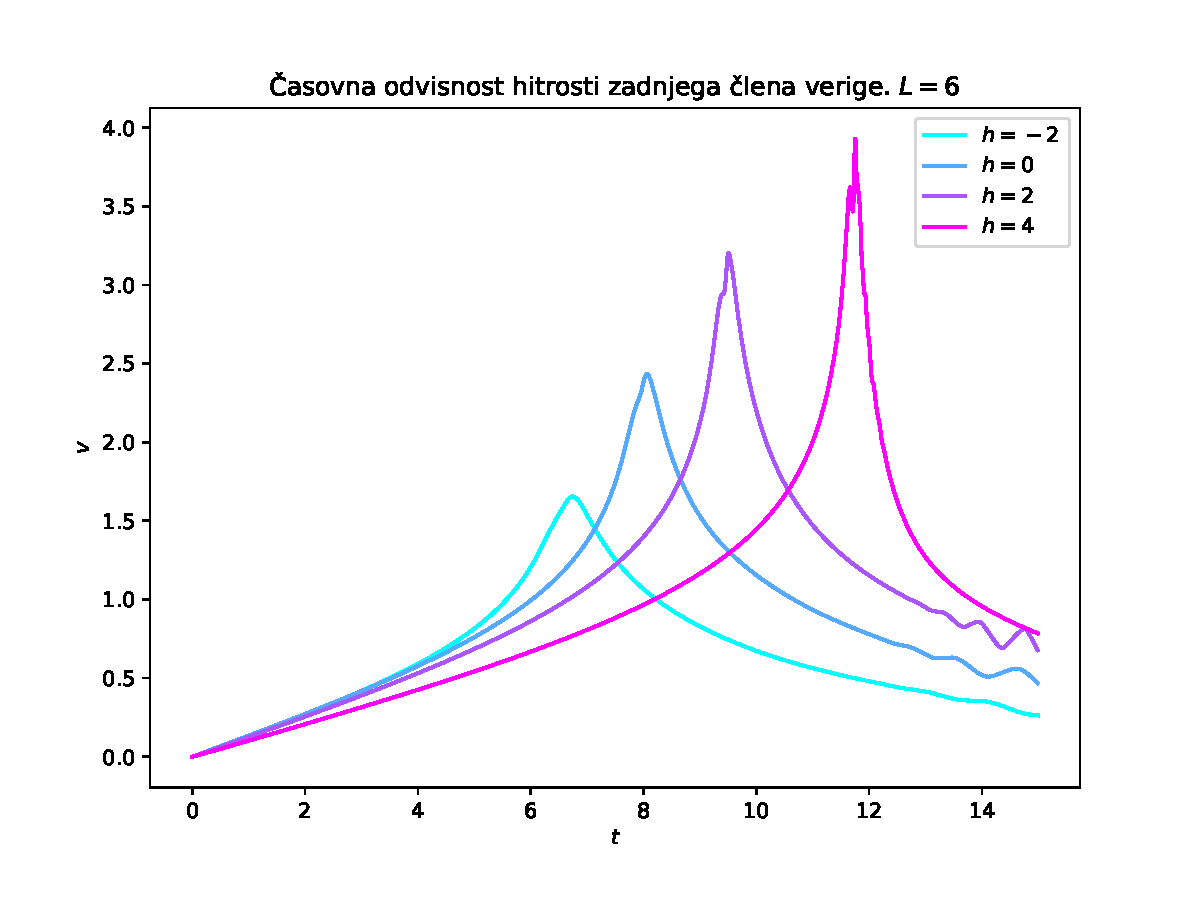
\includegraphics[width=0.95\textwidth]{grafi/hitrost_visoko.pdf}
	\caption{Časovna odvisnost absolutne hitrosti.}
	\label{f:ver-v}
\end{subfigure}
\begin{subfigure}{0.495\textwidth}
	\centering
	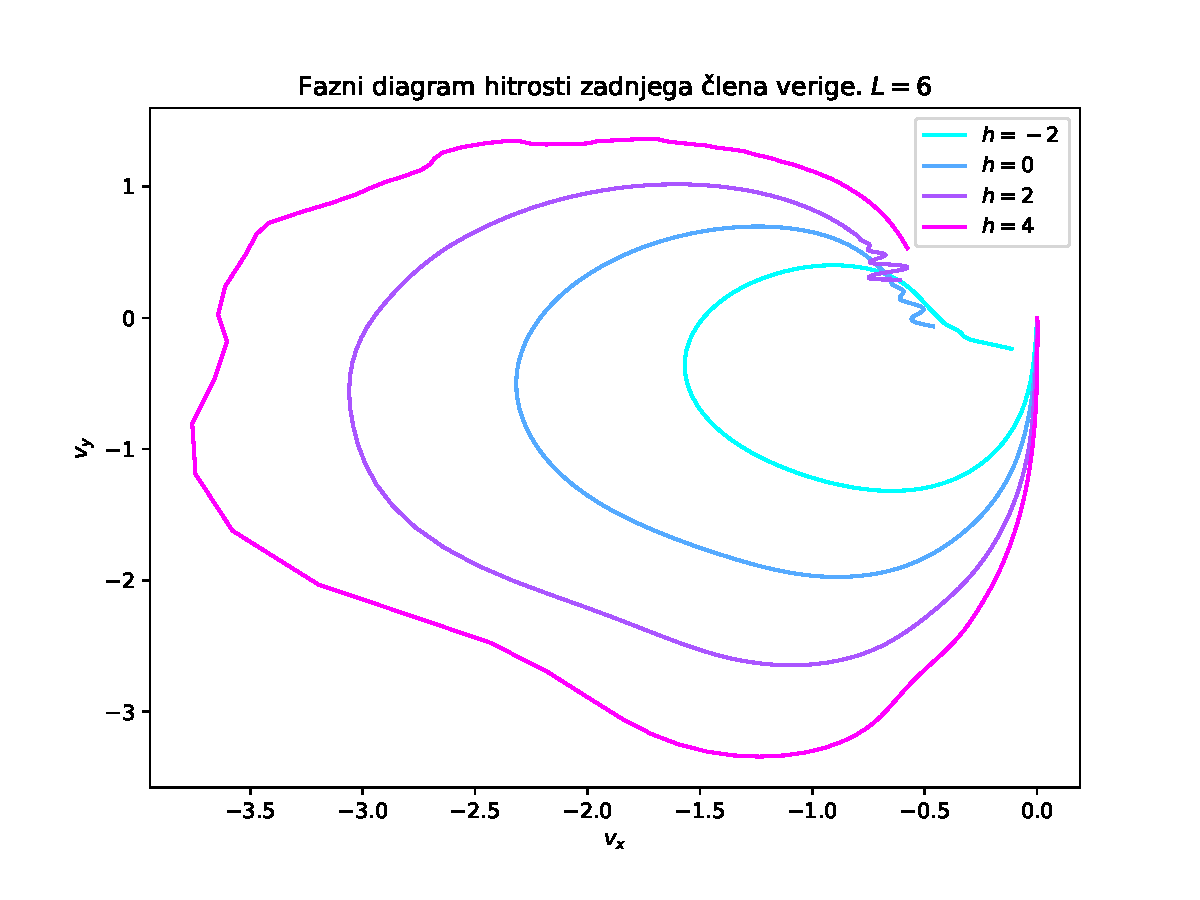
\includegraphics[width=0.95\textwidth]{grafi/hitrost_visoko_xy.pdf}
	\caption{Fazni diagram hitrosti.}
	\label{f:ver-v-fd}
\end{subfigure}
\caption{Hitrost konca vrvi dolžine $L=6$ pri padanju iz različnih višinah desnega sidrišča $h$. Parametri pa so nastavljeni na $r=0.0005$, $m=0.2$, $g=1$. Časovni korak integracije je enak $\diff t = 0.01$. Verigo sestavlja $n=50$ členov.}
\label{f:vertikalno-hitrosti}
\end{figure}


\subsection{Majhen horizontalen razmik med sidriščema}
Začel sem s poskusom, ko je polovica členov verige obrnjenih navzdol, druga polovica pa navzgor. Rezultat je bila veriga, ki se je spustila naravnost v ravnovesno lego, brez da bi kadarkoli šla iz linije $x=0$. Zato sem se odločil za drugačen pristop. Za začetno obliko bom vzel navpično vrv, le da bosta tokrat ${\bi P_0}$ in ${\bi P_1}$ le malenkost zamaknjena tako, da je en člen verige obrnjen vodoravno.

\begin{figure}[H]
\centering
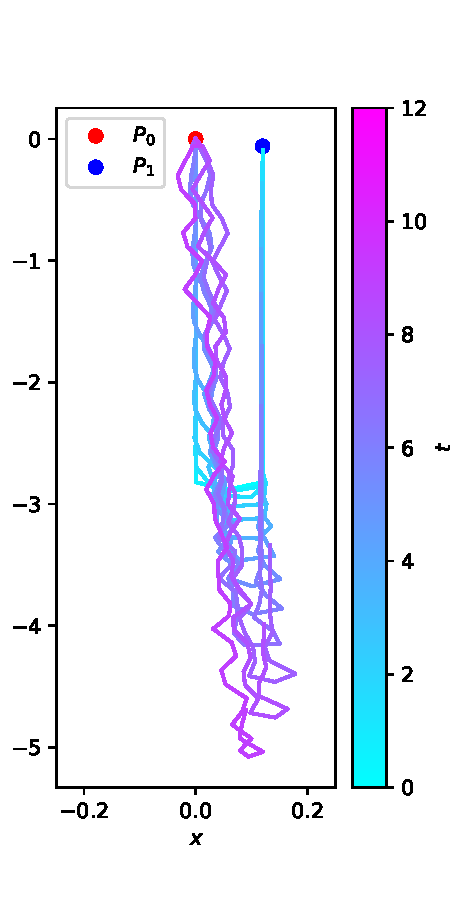
\includegraphics[width=0.2\textwidth]{grafi/vertfall_L.6_n.50_k.1_t.12_r.0.001_m.3_g.1_dt.0.01_freq.75.pdf}
\caption{Potek padanja vrvi, ko sta sidrišči zelo blizu. Parametri pa so nastavljeni na $r=0.001$, $m=0.2$, $g=1$. Časovni korak integracije je enak $\diff t = 0.01$. Verigo sestavlja $n=50$ členov.}
\label{f:skupaj}
\end{figure}

Na sliki \ref{f:skupaj} je prikazano padanje vrvi iz rakega položaja. Dogajanje je povsem drugačno kot v ostalih primerih z večjo razdalo med sidriščima, še posebej ko pride do raztegnjenega stanja. Takrat se zaradi sunkovitega ustavljanja odbije in zmečka. V realnosti naj bi se vrv po tem, ko doseže iztegnjeno stanje spet nazaj dvignila ampak brez hujših premikov v smeri $x$, torej podobno kot simulacija.


\section{Zaključek}
Numerično sem simuliral padanje vrvi ali verige. Obravnaval sem primere, ko je vrv na začetku povsem vodoravna in pa takšne, ko je v obliki črke U z različnimi horizontalnimi in vertikalnimi razmiki med sidriščema. Za problem sem zapisal sistem diferencialnih enačb in jih reševal z uporabo metode Runge-Kutta četrtega reda. Največje težave mi je povzročalo reševanje sistema diferencialnih enačb v primerih, kjer je gibanje vrvi zelo sunkovito, saj je dostikrat kotna hitrost presegla dovoljeni maksimum objekata float. \par\vspace{5mm}

Rezultati simulacij, tako oblike padajoče vrvi kot tudi hitrosti na koncu vrvi, delujejo smiselno in so skladni rezultatom, ki sem jih našel v literaturi \cite{simplechainfall}\cite{tomazevski}. \par\vspace{5mm}

Moja koda je javno dostopna na \href{https://github.com/glotric/falling-chain}{github repozitoriju} \url{https://github.com/glotric/falling-chain}.



\pagebreak
\begin{thebibliography}{9}

\bibitem{simplechainfall}
W. Tomazevski, P.Pieranski. Dynamics of ropes and chains: I. The fall of the folded chain. New Journal of physics, 2005.

\bibitem{tomazevski}
W. Tomazevski, P.Pieranski, J.-C. Germinard. The motion of a freely falling chain tip. American Journal od Physics, 2005



\end{thebibliography}

\end{document}